\chapter{Behoudsvergelijkingen}
\label{sec:Behoudsvergelijkingen}
%%%%%%%%%%%%%%%%%%%%%%%%%%%%%%%%%%%%%%%%%%%%%%%%%%%%%%%%%%%%%%%%%%%%%%%%%%%%%%%%%%%%%%%%%
\begin{toepassing}
	\label{buisaftap}
In een buis met een aftap met afmetingen zoals aangegeven op de figuur stroomt water.
		
Bepaal de gemiddelde stromingssnelheid in de aftap.

	\centering
	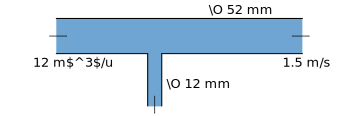
\includegraphics{fig/behoudsvergelijkingen/buisaftap}
\end{toepassing}
\begin{antwoord}{\ref{buisaftap}}
	$v = 1.3\unit{m/s}$
\end{antwoord}
%%%%%%%%%%%%%%%%%%%%%%%%%%%%%%%%%%%%%%%%%%%%%%%%%%%%%%%%%%%%%%%%%%%%%%%%%%%%%%%%%%%%%%%%%
\begin{toepassing}
	\label{afvoerbocht}
Een PVC bochtstuk van 90\deg voor afvoerleiding heeft een binnen diameter van 32mm. De hartlijn heeft een straal van 20mm. Door de buis stroomt water met een debiet van 40l/min.
		
Als er geen drukverliezen optreden in de bocht en de druk aan de uitgang is atmosfeerdruk, bepaal dan de grootte en richting van de kracht die door de stroming uitgeoefend wordt op de buis.

	\centering
	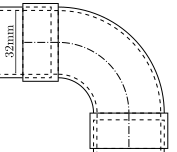
\includegraphics{fig/behoudsvergelijkingen/afvoerbocht}
\end{toepassing}
\begin{antwoord}{\ref{afvoerbocht}}
	$F_x = 0.55\unit{N}$, $F_y = 0.55\unit{N}$
\end{antwoord}
%%%%%%%%%%%%%%%%%%%%%%%%%%%%%%%%%%%%%%%%%%%%%%%%%%%%%%%%%%%%%%%%%%%%%%%%%%%%%%%%%%%%%%%%%
\begin{toepassing}[*]
	\label{waterstraal}
Bereken de kracht die een vrije stationaire waterstraal die loodrecht op een wand spuit op de wand uitoefent.

	\centering
	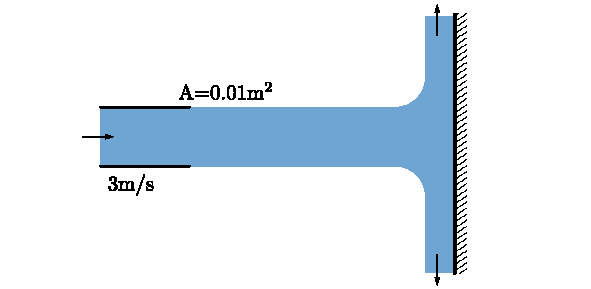
\includegraphics{fig/behoudsvergelijkingen/waterstraal}
\end{toepassing}
\begin{antwoord}{\ref{waterstraal}}
	$F = 90\unit{N}$
\end{antwoord}
%%%%%%%%%%%%%%%%%%%%%%%%%%%%%%%%%%%%%%%%%%%%%%%%%%%%%%%%%%%%%%%%%%%%%%%%%%%%%%%%%%%%%%%%%
\begin{toepassing}[*]
	\label{45gradenbocht}
Een leiding met binnendiameter 300mm ligt in een horizontaal vlak. In de leiding stroomt water aan een debiet van 0.25\unit{m^3/s}.    

Bepaal de grootte en de richting van de kracht die op het bochtstuk inwerkt indien de overdruk voor de bocht 0.4 bar bedraagt. De zwaartekracht mag buiten beschouwing gelaten worden.

	\centering
	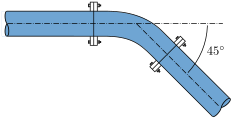
\includegraphics{fig/behoudsvergelijkingen/45gradenbocht}
\end{toepassing}
\begin{antwoord}{\ref{45gradenbocht}}
	$F_x = 1.1\unit{kN}$, $F_y = 2.3\unit{kN}$
\end{antwoord}
%%%%%%%%%%%%%%%%%%%%%%%%%%%%%%%%%%%%%%%%%%%%%%%%%%%%%%%%%%%%%%%%%%%%%%%%%%%%%%%%%%%%%%%%%
\begin{toepassing}[*]
	\label{turbine}
Een hydraulische turbine onttrekt 600MW arbeid aan een waterdebiet van 600\unit{m^3/s}. De inlaat van de turbine heeft een diameter van 8m, de uitlaat een diameter van 10m. Aan de inlaat van de turbine is de druk 10 bar. Het hoogteverschil tussen in- en uitlaat mag verwaarloosd worden.

Bepaal de druk aan de uitlaat van de turbine.

	\centering
	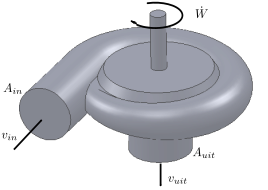
\includegraphics{fig/behoudsvergelijkingen/turbine}
\end{toepassing}
\begin{antwoord}{\ref{turbine}}
	$p = 0.4\unit{bar}$
\end{antwoord}

\section*{Antwoorden}
	\begin{multicols}{2}
		\includecollection{antwoorden}
	\end{multicols}